\chapter[Background]{Background\footnote{Contains text \& images from the Minor Thesis of the author `Business Ideation for \gls{ble}', derived from this thesis' work}} \label{2Back}

This chapter aims at providing a succinct background necessary to understanding the rest of the thesis report. 


Research articles involving the process of porting of Contiki \gls{os} to a hardware platform are presented in section \ref{2Porting}.


\section{\acrlong{ble}}

\subsection{Overview of \gls{ble}}

\acrfull{ble} is a relatively new low power standard incorporated in Bluetooth Core Specification Version 4.0 released by Bluetooth \gls{sig} in 2010\cite{CoreSpec4.0}. This wireless personal area network is marketed as Bluetooth Smart the Bluetooth \gls{sig}. Devices containing only BLE hardware are \emph{single mode} devices, whereas devices containing both classic Bluetooth and BLE are known as \emph{dual mode} devices.   

\gls{ble} was designed by Bluetooth \gls{sig} from the ground up, which helped it achieve certain design goals. These design goals for this wireless personal area network were \emph{low cost, worldwide operation, short range, robustness} and \emph{low power}\cite{Heydon2012}. One most important differentiating factors that has made BLE so successful is the standardization by Bluetooth SIG, facilitating its inclusion in consumer devices and enabling communication across different vendors. In 2013, over 85\% consumer electronic devices supported BLE, making it the de facto standard for low power wireless communication in these devices\cite{Martin2014}. BLE is adopted for various control, notification and monitoring applications, especially in the healthcare, fitness, security and home entertainment industry. 

%\subsection{Design objectives of \gls{ble}}
%
%\paragraph{Low Power} \gls{ble} aims to use a tiny batteries such as button cell to keep a device operating for months to years. To achieve this goal, \gls{ble} was optimized to communicate small amounts of data, such as the states of devices. Also \gls{ble} is optimized to have lower peak power requirements, which allows use of button cells to be used with \gls{ble} devices.
%\paragraph{Worldwide Operation}
%For a technology to be adopted, it is important that there is uniform conformity to the regulations around the world. The 2.4 \si{\GHz} \gls{ism} radio band is the only one available license free worldwide. The technology to develop wireless devices in this band is mature making it the suitable radio band for \gls{ble}.
%\paragraph{Short Range}
%\gls{ble} was designed to be for personal area network like Classic Bluetooth, which means that it is not a network to work with a cellular base station network. This design criterion goes hand in hand with \emph{low power}.
%\paragraph{Low Cost} Lower power requirements mean that the batteries in \gls{ble} devices need to smaller and have to be replaced less frequently, both resulting in a reduction of cost for both the manufacturer and the customer. The use of the \gls{ism} band for communication levels removes the licensing entry barrier for start-ups to develop \gls{ble} devices. \gls{ble} embraces simplicity in its pursuit to lower the cost. \gls{ble} supports only single-hop communication in a star network, which reduces the memory and processor requirement for supporting the protocol. Simplicity was the key factor for the choosing of \gls{gfsk} as the modulation scheme for \gls{ble} to result in low cost, simple implementation of the radio in the \glspl{ic} for \gls{ble}. 
%\paragraph{Robustness} The 2.4~\si{\GHz} space is crowded with devices communicating with various standards as well as spurious noise making the robustness a key criteria in developing \gls{ble} standard. \gls{ble} uses a multi-channel hopping mechanism called \gls{afh} to detect, avoid and recover from interference. In addition to \gls{afh}, \gls{ble} uses \gls{crc} to detect and recover from bit-errors due to background noise.

\subsection[\gls{ble} Network Architecture]{\gls{ble} Network Architecture\cite{BLE101}}

\begin{table}[htbp]
\begin{center}
\begin{tabular}{|m{2.5cm}|m{1.2cm}|m{11.4cm}|}
\hline
\multicolumn{ 2}{|c|}{\textbf{State}} & \textbf{State Description} \\ \hline
\multicolumn{ 2}{|c|}{Standby} & Does not transmit or receive packets, usually sleeping \\ \hline
\multicolumn{ 2}{|c|}{Advertising} & Broadcasts advertisement packets in  advertising channels \\ \hline
\multicolumn{ 2}{|c|}{Scanning} & Looks for advertisement packets, across advertising channels \\ \hline
\multicolumn{ 2}{|c|}{Initiating} & Initiates connection to advertiser to get Master role \\ \hline
\multicolumn{ 1}{|c|}{Connection} & Master & Communicates with device(s) in the \emph{slave} role, defines configuration of the connection \\ \cline{ 2- 3}
\multicolumn{ 1}{|l|}{} & Slave & Communicates with a single device in \emph{master} role \\ \hline
\end{tabular}
\end{center}
\vspace{-12pt}
\caption{Possible states of a BLE device}
\vspace{-6pt}
\label{tbl:BLEstates}
\end{table}

Table \ref{tbl:BLEstates} shows the possible states of a BLE device and figure \ref{fig:Roles} illustrates the ways in which these states can change. The standby role is universally supported across all BLE devices and the other roles are present in device according to their configuration. For example, a device with only a radio transmitter can alternate between the advertising and standby state, usually called an \emph{advertiser}. Similarly a \emph{scanner} can just receive BLE packets.

\begin{wrapfigure}{r}{0.55\textwidth}
\centering
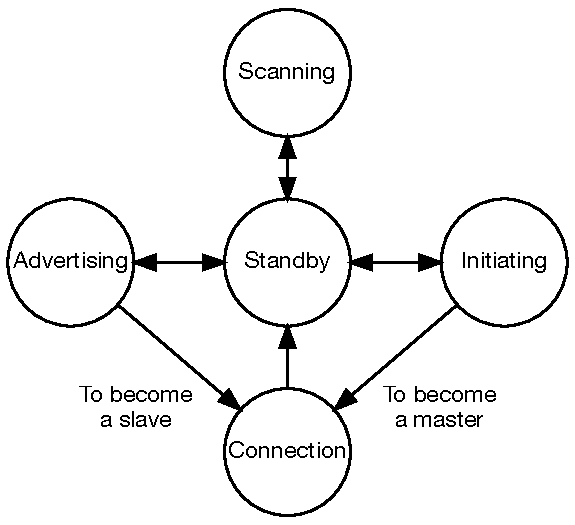
\includegraphics{Roles.pdf}
\caption{State diagram of BLE states}
\label{fig:Roles}
\vspace{-10pt}
\end{wrapfigure}

A connection can be formed between two BLE devices, with the master node reaching from the initiating state and the slave node from the advertising state. This master and slave roles follows an asymmetric design philosophy. A slave is a simple device that can be connected with at most one master at a time and are usually single purpose devices. A master on the other hand is a more complex device which is responsible for coordinating the connections and activities of all the slaves connected to it. A master is usually a multi-purpose device such as a mobile phone, tablet or a laptop. A master connected with multiple slaves employs a star topology. The slaves cannot directly communicate with each other. An example of a BLE network is shown in figure \ref{fig:TopoBLE}. Here a master can be seen connected to multiple slaves. The bidirectional continuous lines show data communicated in both directions when in a connection. The dashed lines show the data from the advertisements being sent broadcast. A master or slave can be an advertiser simultaneously as seen in the figure \ref{fig:TopoBLE}.  

\begin{figure}[h]
\centering
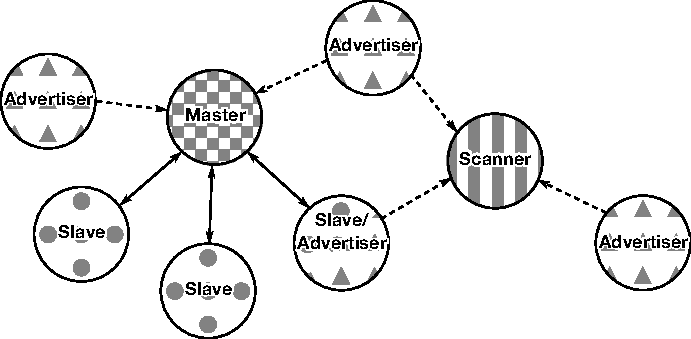
\includegraphics{TopologyBLE.pdf}
\caption{An example of BLE topology}
\label{fig:TopoBLE}
\end{figure}

%\begin{figure}[h] %{r}{0.51\textwidth}
%%\vspace{-15pt}
%  \begin{center}
%	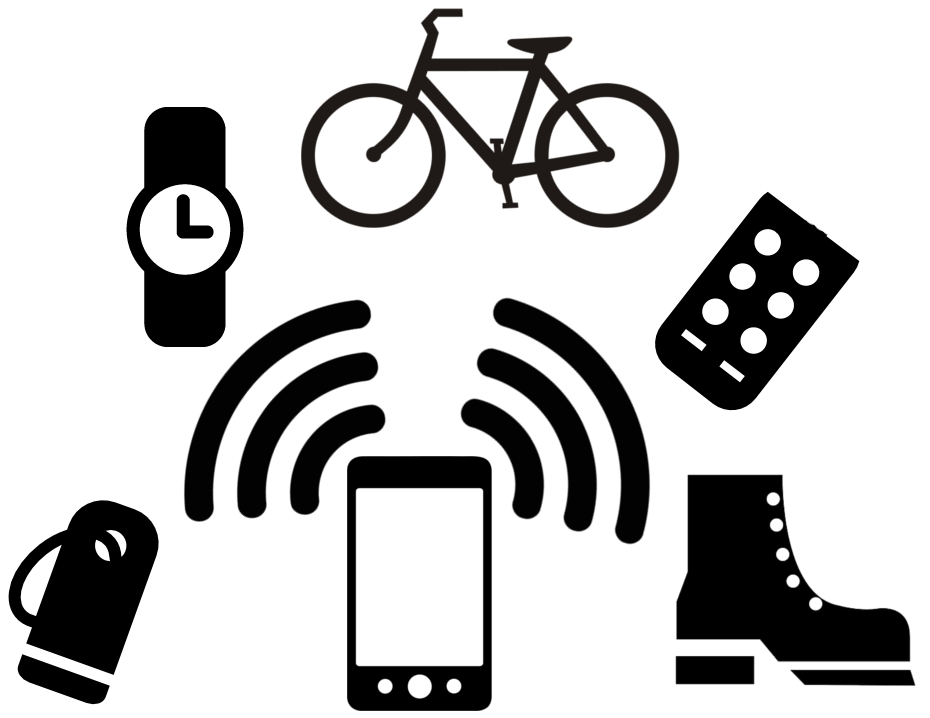
\includegraphics[width=0.49\textwidth]{devicesBLE}
%  \end{center}
%\caption{Typical BLE network}
%%\vspace{-10pt}
%\label{devicesBLE}
%\end{figure}

\section[\gls{ble} stack overview]{\gls{ble} stack overview\cite{Heydon2012}}

To implement the BLE network described in the previous section, the BLE stack used is as shown in figure \ref{fig:StackBLE}. The BLE stack is split into a host section and a controller section. The controller part takes care of the actual interaction with the radio and enforcing the timing requirements. The controller part is implemented in the \gls{ic} where the radio is located, usually the \gls{soc} or the discrete transceiver. On the other hand, the host contains the software required for handling the various kinds of BLE packets. This separation of host and controller allows mixing and matching of these parts from different sources. The communication between the host and controller is done through the Host Controller Interface.

\begin{figure}[h]
\begin{center}
\begin{tabular}{|c||c|c|}
\cline{2-3}
\multicolumn{1}{c|}{} &  \multicolumn{ 2}{c|}{Applications} \\ \hline
\multicolumn{ 1}{|c||}{} & \multicolumn{ 2}{c|}{Generic Access Profile} \\ \cline{ 2- 3}
\multicolumn{ 1}{|c||}{Host} & \multicolumn{ 2}{c|}{Generic Attribute Profile} \\ \cline{ 2- 3}
\multicolumn{ 1}{|l||}{} & \multicolumn{1}{c|}{Attribute Protocol} & \multicolumn{1}{c|}{Security Manager} \\ \cline{ 2- 3}
\multicolumn{ 1}{|l||}{} & \multicolumn{ 2}{c|}{Logic Link Control and Adaptation Protocol} \\ \hline \cline{2-3}
\multicolumn{1}{c|}{} & \multicolumn{ 2}{c|}{Host Control Interface} \\ \cline{2-3} \hline
\multicolumn{ 1}{|c||}{} & \multicolumn{1}{c|}{Link Layer} & \multicolumn{1}{c|}{Direct Test Mode} \\ \cline{ 2- 3}
\multicolumn{ 1}{|c||}{Controller} & \multicolumn{ 2}{c|}{Physical Layer} \\ \hline
\multicolumn{ 1}{c}{} & \multicolumn{1}{m{4cm}}{} & \multicolumn{1}{m{4cm}}{} \\ 
\end{tabular}
\end{center}
\vspace{-30pt}
\caption{BLE Stack}
\label{fig:StackBLE}
\end{figure}

\paragraph{Physical layer}
This is layer with the actual task of sending and receiving electromagnetic signals with a 2.4 GHz \gls{ism} radio. The modulation scheme used is \gls{gfsk}. There are 40 channels over which BLE operates, each 2 MHz apart from each other. In these there are 3 advertisement channels for sending advertisement packets. These are spread over the \gls{ism} band, located where overlapping with WiFi signals does not occur. The rest of the channels are used for communicating data when in connection mode.

\paragraph{Link layer}


\paragraph{\gls{l2cap}} This layer is responsible for multiplexing data from different logical channels in BLE, although in Bluetooth 4.0 only three fixed channels are used. 

\paragraph{Security Manager} This layer is used for pairing BLE devices, which is a form of authenticating the other device. Typically this is followed by encryption key distribution.

\paragraph{\gls{att}} This layer defines the \emph{Client-Server} architecture used by BLE to communicate data. A server is where data is held in a database and a client is one which gets the data from a server. All data stored in BLE devices as \emph{Attributes}, which is data organized in a specific format containing a label and address. Thus, a client can requests and gets a specific attribute from a server's database. Client or server configuration is independent of the role in link layer. A master or slave device can have \emph{both} a client and a server.

Attributes can be accessed from the attribute database in six ways as listed below.

\begin{easylist}[itemize]
& Find Requests: Client can find the attributes present in server's database.
& Read Request: Clients requests to get an attribute in server, to which the server responds with the requested attribute.
& Write Request: Client writes to an attribute in server with acknowledgment back.
& Write Command: Client writes to an attribute in server without acknowledgment back.
& Notification: Unprompted by the client, server sends an attribute to a client, to which the client does not acknowledge.
& Indication: Unprompted by the client, server sends an attribute to a client, to which the client acknowledges.
\end{easylist}

\paragraph{\gls{gatt}}
This layer organizes the attributes in a hierarchical manner, so that similar attributes can be encapsulated together.

\paragraph{\gls{gap}}
This layer defines how BLE devices discover, connect and present useful information to the users and each other. A device having peripheral \gls{gap} role advertises and then connects to become a slave at link layer. A \gls{gap} central device initiates connection to a peripheral and becomes a master at link layer once connected.

\section{Overview of Contiki}
??????????????? Which aspects of Contiki here?


\subsection{Porting the Contiki \gls{os} to a New Platform} \label{2Porting}
Contiki \gls{os} project originating in 2002 has been ported to an increasing number of hardware platforms \cite{contikiHw}. Since Contiki is an open-source BSD Clause-3 licensed project, there are many projects in various hardware platforms based on a fork from the Contiki repository.

These hardware platforms' processors range across a spectrum of 8-bit (8051 and AVR), 16-bit (MSP430) to 32-bit (ARM Cortex-M, PIC32). Contiki has support for 802.15.4 based wireless communication with various external transceivers and \glspl{soc} with built in radio transceiver. Various common features of many platforms such as \glspl{led}, buttons and serial port have modules in Contiki for common \gls{api} across platforms.

In \cite{Oikonomou2011} the authors describe Contiki's port to a CC2430 based platform manufactured by Sensinode Ltd. CC2430 is an enhanced Intel 8051 processor based \gls{soc} having 802.15.4 physical layer compatible radio transceiver. The authors fully debugged the port which had of a code footprint of about 100 kB, varying based on the compiler mode and the features enabled. Many new features were added to the port including support for \gls{adc} unit, all the sensor available on the platform (accelerometer, light sensor, voltage and temperature sensors), watchdog timer and the general purpose buttons. Because of the limited stack availability of 233 bytes, many optimizations such as moving variables to external \gls{ram} memory space and re-writing the radio driver for CC2430 to prevent stack from overflowing.

Contiki was ported to two new platforms, namely MicaZ and TelosB in a Bachelor thesis \cite{stan2007porting}. TelosB, similar to the TMote-Sky platform, consists of a 8MHz 16-bit MSP430 \gls{mcu}, a CC2400 transceiver with 802.15.4 \gls{phy} and a host of sensors to measure light, temperature and humidity. The port to TelosB was done by changing the port to the fully supported TMote-Sky platform. MicaZ platform consisted of a 8-bit Atmel ATMega128L \gls{mcu} and a CC2400 transceiver. MicaZ platform needed rewriting of the code for processor abstraction so that the high level Contiki \glspl{api} could work.

Contiki has been ported into platform based on a ARM Cortex M3 processor to create a device wired with Ethernet to connected to the Internet \cite{Wilde2013a}. Ethernet based networking with the libraries present in Contiki was developed in this project to demonstrate as a proof of concept. There are many unofficial ports of Contiki to various hardware platforms.

\section{Overview of 802.15.4}
Mention that in this thesis the Contiki specific implementations of the 802.15.4 layers will be tested.

\subsection{Physical layer}

\subsection{\gls{mac} layer}

The link layer of 802.15.4 consists of \gls{mac} layer on top of a \gls{rdc} layer. For the RDC layer the Null-RDC and ContikiMAC driver will be tested in each of the test with \gls{csma} as the \gls{mac} layer. In case of Contiki-MAC the receiving node switches on periodically to sense if there are any packets that need to be received. The default time of this period is 125 ms. In case of null-RDC the radio receiver is never switched off, as the name suggests.


\subsubsection{\gls{rdc} layer}
\subsubsection{\gls{csma}}


